\documentclass[]{article}
\usepackage{graphicx}
\usepackage{caption}
\usepackage{ragged2e}
\graphicspath{{plots/}}

%opening
\title{\vspace{0.0001mm}Comparison UUnifast and DRS}
\author{Souvik Sarkar and Mario Günzel}

\renewenvironment{abstract}
 {\par\noindent\textbf{\abstractname:}\ \ignorespaces}
 {\par\medskip}

\begin{document}
	
	\maketitle
	
	\begin{abstract}
 
{
\raggedleft This is a short comparison of the evaluation results obtained from UUnifast and from DRS.
}
	\end{abstract}
 
\paragraph{UUniFast:} \hspace{0pt} \\

{\raggedleft For UUniFast suspension time ['sslength'] is drawn uniformly from the interval between the minimum suspension length value and maximum suspension length value. We have the following three setups:
}
 
 \begin{itemize}
		\item Setup 1 Short Suspension [0.0(Ti - Ci), 0.2(Ti - Ci)]
		\item Setup 2 Moderate Suspension [0.2(Ti - Ci), 0.4(Ti - Ci)]
		\item Setup 3 Long Suspension [0.4(Ti - Ci), 0.6(Ti - Ci)]
\end{itemize}



\paragraph{DRS:} \hspace{0pt} \\

{\raggedleft 
Unlike UUniFast, Dirichlet- Rescaling Algorithm are used for asymmetric constraints and works with separate upper bounds and lower bounds for each task. 
}

The three different setups for DRS used here:
	
	\begin{itemize}
		\item Setup 1 (minsus+ex=0.1*number of tasks per set, maxsus+ex=1.0)
		\item Setup 2 (minsus+ex=0.3*number of tasks per set, maxsus+ex=1.0)
		\item Setup 3 (minsus+ex=0.5*number of tasks per set, maxsus+ex=1.0)
	\end{itemize}

{\raggedleft
Here, we are taking three different setups each with different execution + suspension time but same execution time.
}
% ======================
	\clearpage

\section{Suspension Oblivious}

{
\raggedleft We are going to generate a suspension-oblivious schedule for the DRS
}

{
\raggedleft and UUniFast setups explained above
}

	
	\begin{minipage}[t]{0.48\linewidth}
		\centering
		\textbf{(UUnifast)}
		\vspace{0.3cm}
		
		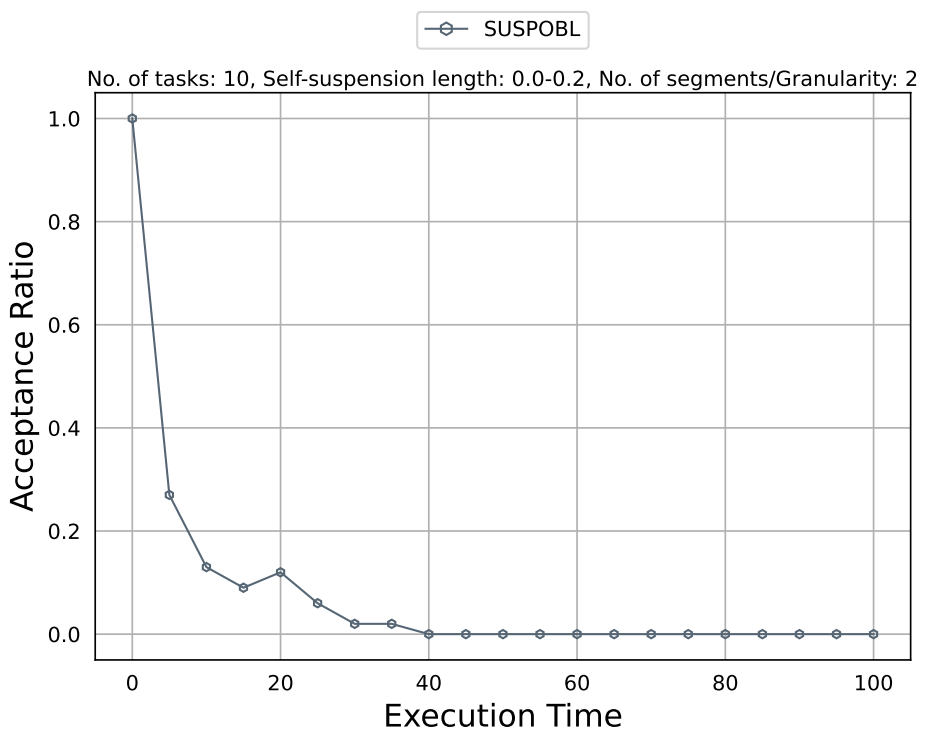
\includegraphics[width=\linewidth]{Capture.png}
		First UUnifast setup.

  
		\vspace{0.3cm}
		
		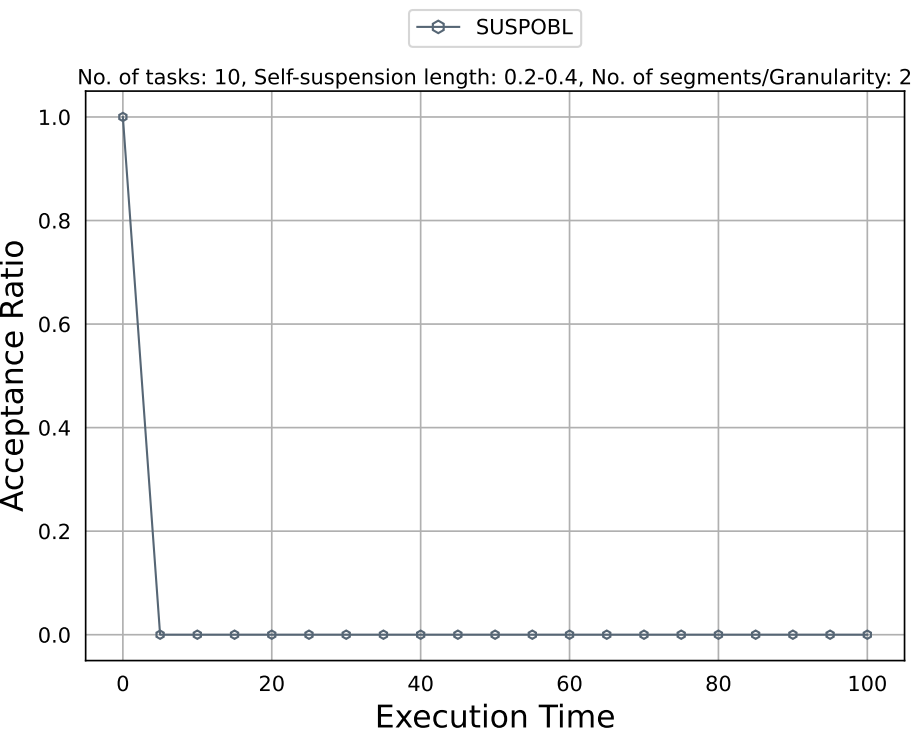
\includegraphics[width=\linewidth]{Capture2_uunifast.png}
		Second UUnifast setup.
		\vspace{0.3cm}
		
		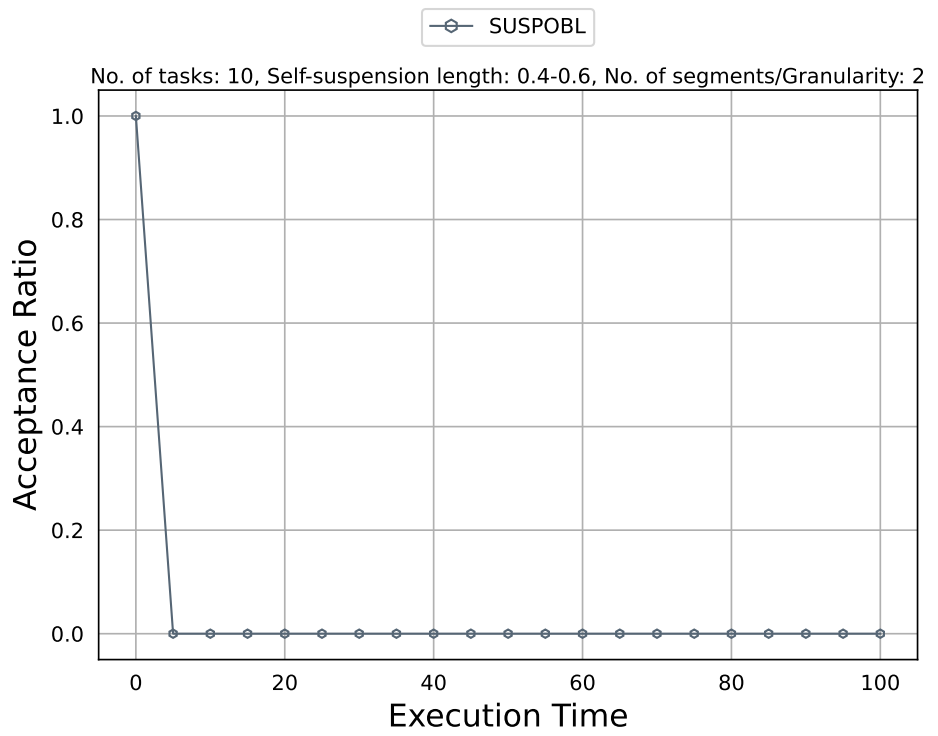
\includegraphics[width=\linewidth]{Capture3_uunifast.png}
		Third UUnifast setup.
		\vspace{0.3cm}
		
		
	\end{minipage}\hfill
	\begin{minipage}[t]{0.48\linewidth}
		\centering
		\textbf{(DRS)}
		\vspace{0.3cm}
		
		\includegraphics[width=\linewidth]{Capture1_DRS.png}
		First DRS setup.
		\vspace{0.3cm}
		
		\includegraphics[width=\linewidth]{Capture2_DRS.png}
		Second DRS setup.
		\vspace{0.3cm}
		
		\includegraphics[width=\linewidth]{Capture3_DRS.png}
		Third DRS setup.
		\vspace{0.3cm}
	\end{minipage}

% ======================
	\clearpage
	\section{Suspension Jitter}
{
\raggedleft We are going to generate a suspension-jitter schedule for the DRS
}

{
\raggedleft and UUniFast setups explained above
}


	
	\begin{minipage}[t]{0.48\linewidth}
		\centering
		\textbf{(UUnifast)}
		\vspace{0.3cm}
		
		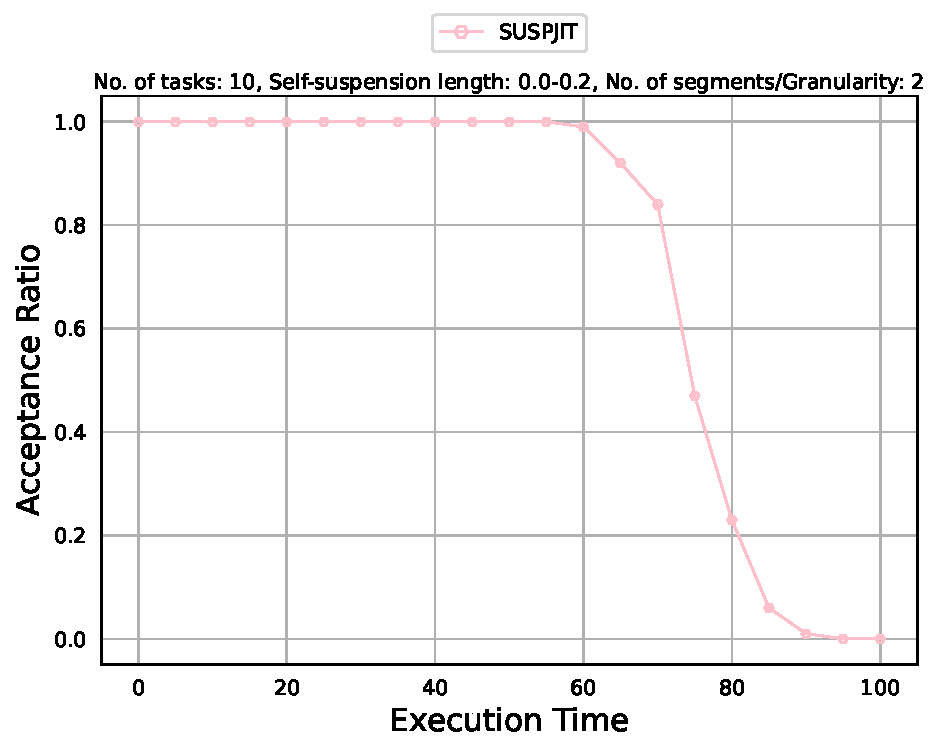
\includegraphics[width=\linewidth]{SUSPJIT[2][0.0-0.2][10].pdf}
		First UUnifast setup.
		\vspace{0.3cm}
		
		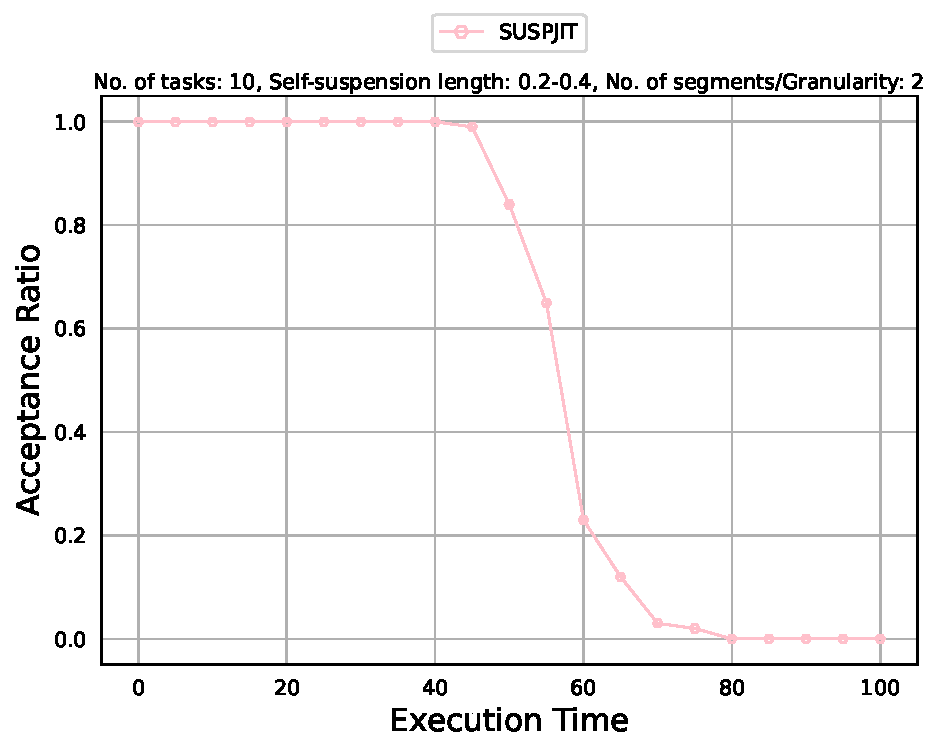
\includegraphics[width=\linewidth]{SUSPJIT[2][0.2-0.4][10].pdf}
		Second UUnifast setup.
		\vspace{0.3cm}
		
		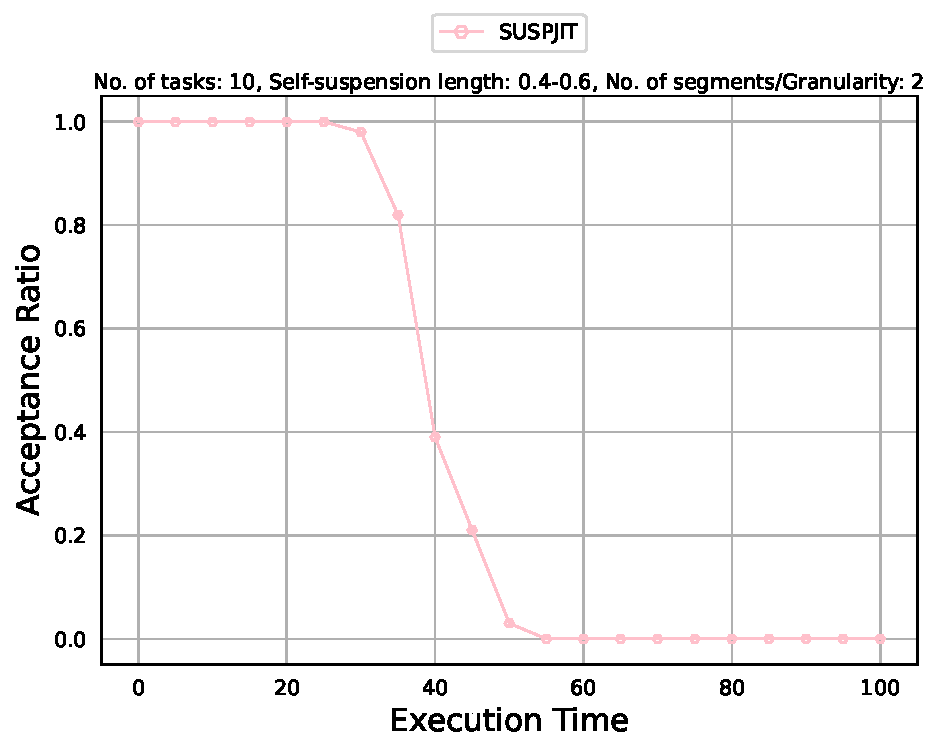
\includegraphics[width=\linewidth]{SUSPJIT[2][0.4-0.6][10].pdf}
		Third UUnifast setup.
		\vspace{0.3cm}
		
		
	\end{minipage}\hfill
	\begin{minipage}[t]{0.48\linewidth}
		\centering
		\textbf{(DRS)}
		\vspace{0.3cm}
		
		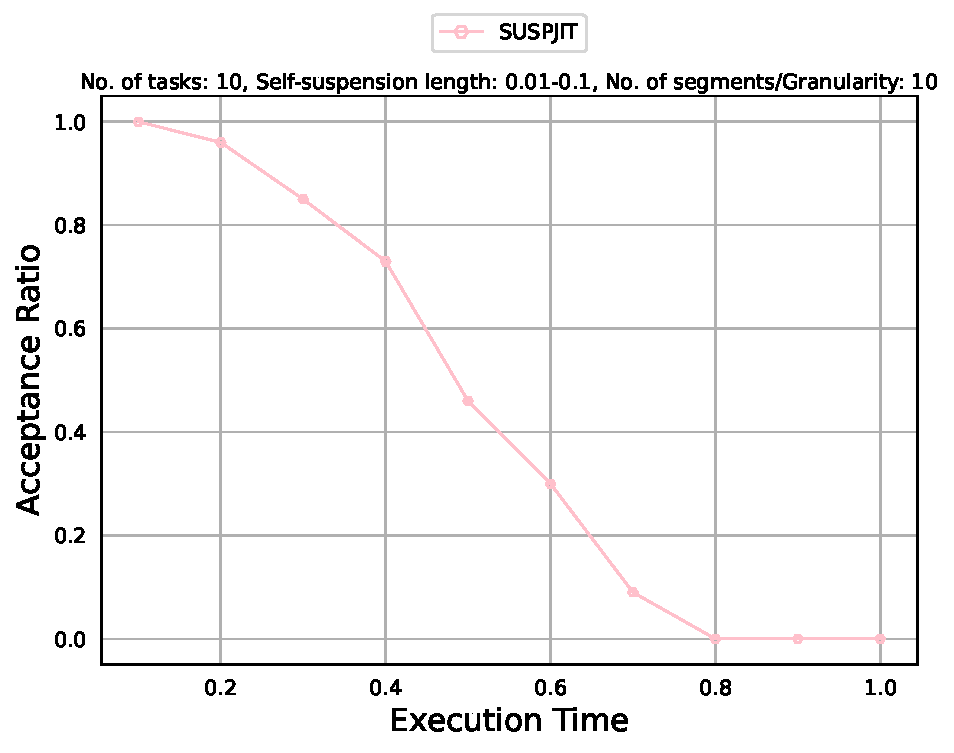
\includegraphics[width=\linewidth]{SUSPJIT_First Setup.pdf}
		First DRS setup.
		\vspace{0.3cm}
		
		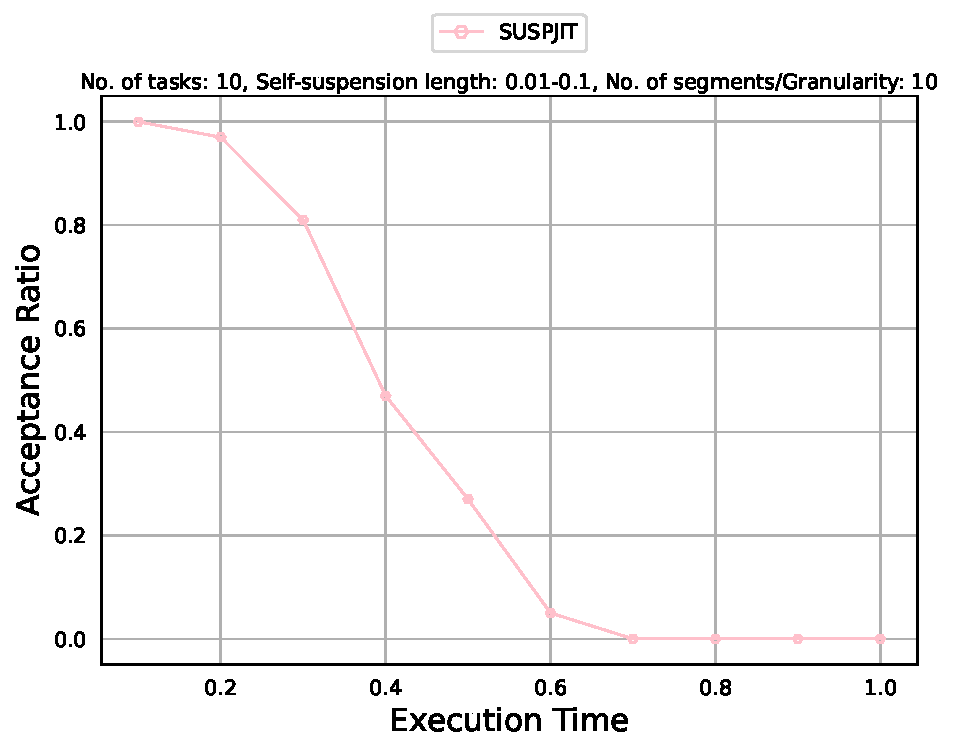
\includegraphics[width=\linewidth]{SUSPJIT_Second Setup.pdf}
		Second DRS setup.
		\vspace{0.3cm}
		
		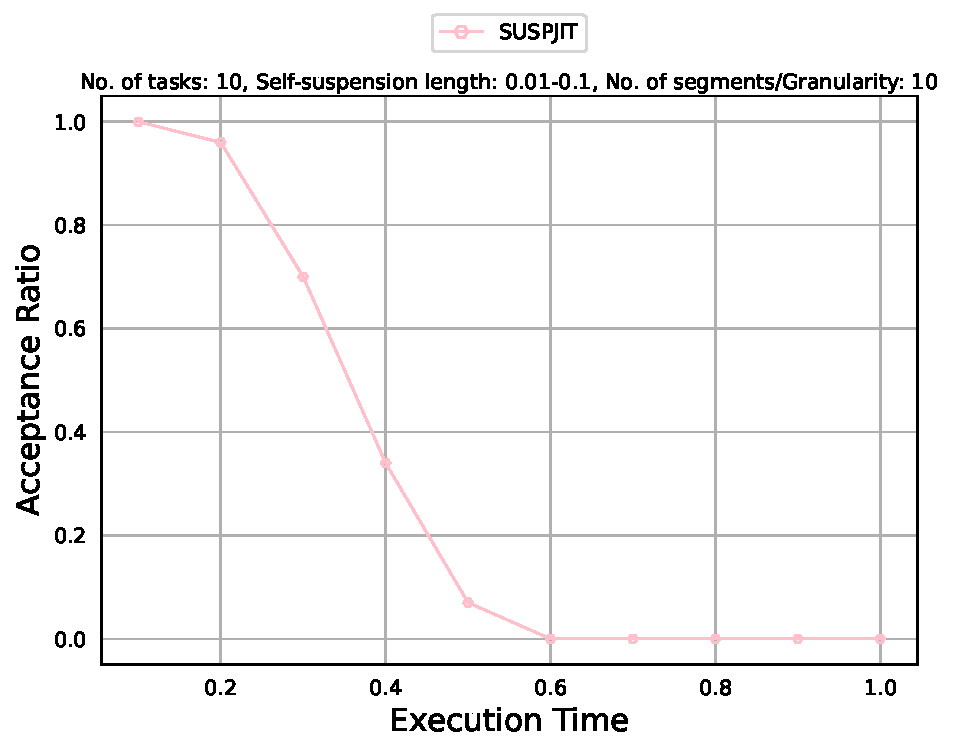
\includegraphics[width=\linewidth]{SUSPJIT_3rd Setup.pdf}
		Third DRS setup.
		\vspace{0.3cm}
	\end{minipage}

\paragraph{Evaluation:} \hspace{0pt} \\

{
\raggedleft So, the parameter we use to comapare is \textbf{Acceptance Ratio} with respect to the execution time i.e the percentage of tasksets that got accepted for a particular execution time. We are generating 100 task sets per configuration with 10 tasks per set with a suspension values ranging between 0,0 - 0,6. \newline
}


{
\raggedleft
We use two methods DRS and UUniFast to generate a set of utilization values with motive of generating (Usum, ubound, lbound) and (Usum) respectively. The resulted tasksets were then tested under \textbf{Suspension Oblivious} and \textbf{Suspension Jitter}. We see in the resulting graphs (above) that Acceptance Ratio gets reduced for tasksets with higher suspension intervals. \newline 
}

{
\raggedleft
Using Suspension oblivious methods we see a higher acceptance ratio for taskets generated using DRS over UUniFast method. But, we also see that those same DRS task sets acheive a slightly lower acceptance ratio using Suspension Jitter schedule. 
}
\end{document}
